\chapter{Soluzione di Schwarzschild}\label{para.schwarz}
Questa soluzione, proposta da Karl Schwarzschild nel 1916 pochi mesi dopo la pubblicazione della stessa relatività generale da parte di Einstein, rappresenta la prima soluzione nota alle equazioni di campo.

Essa permette la descrizione dello spaziotempo dovuto ad una distribuzione di massa sfericamente simmetrica, non rotante, non pulsante e priva di carica. In buona approssimazione, in quanto gli stessi corpi celesti ruotano, permette la descrizione dei moti planetari tra cui quello del nostro sistema solare. Oltre all'importanza storica dell'essere la prima soluzione, la sua applicabilità ha permesso le prime verifiche della teoria attraverso quelli che sono noti come \emph{test classici} della relatività generale: la precessione dell'orbita di Mercurio, la deviazione dei raggi di luce, il redshift gravitazionale, la dilatazione temporale.
Nondimeno introduce per la prima volta il concetto di buco nero, quale singolarità della metrica dello spaziotempo.

\section{Metrica di Schwarzschild}
Per l'ottenimento della soluzione, vogliamo determinare le metriche statiche e sfericamente simmetriche tali che soddisfino
\begin{equation*}
    R_{\mu\nu}=0
\end{equation*}
o come si usa dire, con \virgolette{Ricci piatto}. La soluzione è quindi cercata nel vuoto.
\begin{definizione}
Uno spaziotempo $\mathcal{M}$ viene chiamato \textbf{stazionario} se esiste un gruppo di isometrie $\phi_t$, parametrizzate in $t$, le cui orbite sono curve di tipo tempo. 
\end{definizione}
Questo gruppo di simmetrie esprime la simmetria dello spaziotempo sotto traslazione del tempo, ovvero possiede un vettore di Killing $\xi$ di tipo tempo.
Come maggiore conseguenza si ha che con tale parametro \textbf{la metrica non dipende dal tempo}.
\begin{definizione}
Uno spaziotempo $\mathcal{M}$ viene detto \textbf{statico} se è stazionario e se esiste una ipersuperficie $\Sigma$ (tipo spazio) ortogonale alle orbite dell'isometria.
\end{definizione}

Se il vettore di Killing $\xi\neq0$ su tutto $\Sigma$, allora ogni punto in un intorno dell'ipersuperficie giace in una e una sola orbita di $\xi$ passante per $\Sigma$.  Scegliamo $x^i$ come coordinate sulla ipersuperficie $\Sigma$; assegniamo a $p$ le coordinate $(t,x^i)$, dove $t$ è parametro dell'orbita, che parte da $\Sigma$ e finisce nel punto $p$, e $x^i$ le coordinate del punto iniziale su $\Sigma$ ovvero dell'intersezione tra l'orbita e l'ipersuperficie. Come visto, siccome $\partial_t$ è un vettore di Killing che coinvolge il parametro di Killing, allora la metrica sarà indipendente dal tempo; inoltre poiché $\Sigma_t$ (insieme di punti a fissato $t$) è immagine di $\Sigma$ sotto l'isometria, si avrà $\Sigma_t \perp \xi$.\footnote{In altre parole lo spaziotempo statico ha una forma locale del tipo $\mathcal{M}= \mathbb{R}\times \Sigma.$}

Questo comporta che la metrica statica più generale è:
\begin{equation*}
    ds^2 =- V(x^1,x^2,x^3)dt^2 + \sum_{i,j=1}^3 h_{ij}(x^1,x^2,x^3)dx^i dx^j
\end{equation*}
Osserviamo che i termini misti $dtdx^i$ sono assenti proprio per l'ortogonalità detta tra $\partial_t$ e $\Sigma$. Diversamente una metrica stazionaria, ma non statica dovrà per forza aver questi termini misti in un qualsiasi sistema di coordinate che coinvolge il parametro di Killing.

In aggiunta osserviamo che il diffeomorfismo che porta $t \mapsto -t$ (riflessione temporale) è anch'esso una isometria nella metrica statica qui sopra. In aggiunta al diffeomorfismo di traslazione temporale $t \mapsto t + c$ che è isometria per tutti gli spazitempo stazionari, uno spaziotempo statico gode in più di questa simmetria. Fisicamente non è detto che i campi che godono di simmetria tempo-traslazionale, godano anche di simmetria per riflessioni del tempo, basti pensare ad un moto rotatorio che in tal caso invertirebbe il verso di rotazione, non preservando l'invarianza.

La metrica stazionaria più generale è invece:
\begin{equation*}
    ds^2 = -V(x^1,x^2,x^3)dt^2 + \sum_{i,j=1}^3 h_{ij}(x^1,x^2,x^3)dx^i dx^j + \sum_{i=1}^3 a_{i}dx^idt
\end{equation*}
\begin{definizione}
Uno spaziotempo $\mathcal{M}$ è \textbf{sfericamente simmetrico} se il suo gruppo di isometrie contiene un sottogruppo isomorfo a $SO(3)$ con orbite che sono 2-sfere.
\end{definizione}
Le isometrie di $SO(3)$ possono essere interpretate come rotazioni e pertanto un tale spaziotempo possiede metrica invariante sotto rotazioni. La metrica dello spaziotempo induce una metrica su ciascuna delle 2-sfere (che ricordiamo essere le orbite) che, a causa della simmetria rotazionale, sarà proporzionale a quella della 2-sfera unitaria.

In un sistema di coordinate sferico, ciascuna delle metriche sulle 2-sfere assumerà la forma:
\begin{equation}
    ds^2 = r^2(d\theta^2 + \sin^2\theta d\phi^2)
\end{equation}

Nell'ipotesi di uno spaziotempo statico e sfericamente simmetrico, se il vettore di Killing di tipo tempo $\xi$ è unico, sarà ortogonale alle 2-sfere; infatti essendo unico, deve essere invariante sotto simmetrie rotazionali e perciò le proiezioni su ogni sfera di orbita dovranno essere nulle. Questo comporta che le 2-sfere giacciano completamente nelle ipersuperfici $\Sigma_t$ (che sono ortogonali a $\xi_t$).
Scegliendo $(r,\theta,\phi)$ come coordinate\footnote{$r$ non assume necessariamente il significato di distanza dal centro in quanto un centro può anche non esistere. \'E il caso per esempio della topologia $\mathbb{R}\times S^2$. Nonostante ciò si tende comunque a chiamare coordinata radiale $r$.} sull'ipersuperficie $\Sigma$, la metrica assume la forma:
\begin{equation*}
    ds^2 = -f(r)dt^2 + h(r)dr^2 +r^2(d\theta^2 + \sin^2\theta d\phi^2)
\end{equation*}
che rappresenta la più generale metrica statica e sfericamente simmetrica. Come gruppo di isometrie ha $\mathbb{R}\times SO(3)$.

Imponiamo ora le equazioni di Einstein con il Ricci piatto, $R_{\mu\nu}=0$ (sono omessi i calcoli):
\begin{align*}
    R_{tt}=0 &\implies \frac{1}{2} (fh)^{-1/2}[(fh)^{-1/2}f']' + \frac{f'}{rfh} = 0 \\
    R_{rr}= 0 &\implies -\frac{1}{2}(fh)^{-1/2}[(fh)^{-1/2}f']' + \frac{h'}{rh^2} = 0 \\
    R_{\theta\theta}=0 &\implies -\frac{1}{2}\frac{f'}{rfh}+\frac{1}{2}\frac{h'}{rh^2} + r^{-2}(1-h^{-2}) = 0
\end{align*}
L'equazione $R_{\phi\phi}=0$ implica la stessa di $R_{\theta\theta}$ proprio per la simmetria rotazionale. Risolviamo sommando le prime due:

Pertanto la metrica statica e sfericamente simmetrica ottenuta con le equazioni di Einstein é:
\begin{equation}
    ds^2 = -\left( 1+ \frac{C}{r}\right)dt^2 + \frac{1}{1+ \frac{c}{r}}dr^2 +r^2(d\theta^2 + \sin^2\theta d\phi^2)
    \label{eq.metricageneraleschwarz}
\end{equation}

Per prima cosa osserviamo che per $r \rightarrow +\infty$, la metrica tende a quella piatta di Minkowski (si usa dire \textit{asintoticamente piatta}) e ciò ci permette di usare questo tipo di metrica per descrivere il comportamento a grandi distanze come se fosse un campo gravitazionale generato da un corpo isolato.

Secondariamente, ma non per importanza, riportiamo un teorema, senza dimostrazione:
\begin{teorema}[di Birkhoff]
Ogni soluzione a simmetria sferica delle equazioni di campo di Einstein nel vuoto, è statica.
\end{teorema}
Questo teorema comporta che le equazioni di Einstein possono essere risolte per un generico spaziotempo a simmetria sferica senza assumere necessariamente la staticità dello stesso.
Nonostante ciò è dimostrato (vedi \cite{hawking}) che la soluzione di Schwarzschild rimane l'unica soluzione di questo più generale problema di equazioni; pertanto tutte le soluzioni nel vuoto con spazitempo sfericamente simmetrici e con $R_{\mu\nu}=0$ sono statiche. O equivalentemente, la soluzione di Schwarzschild è l'unica soluzione sfericamente simmetrica nel vuoto per la relatività generale.

Il valore della costante può essere determinato paragonando il moto di un corpo test in regime di gravità debole all'equazione di Newton. Riprendendo i calcoli già effettuati in \S\ref{para.limitenewton}:
\begin{equation*}
    \frac{d^2 x^i}{dt^2}= - \tensor{\Gamma}{^i_{tt}} = - \frac{\partial \phi}{\partial x^i}
\end{equation*}
Stabiliamo quindi il collegamento tra la teoria newtoniana, sapendo che $\phi= -\frac{M}{r}$, con la relatività calcolando il coefficiente con la gravità linearizzata e imponendo la corrispondenza tra le due:
\begin{equation*}
    \Gamma_{itt}= \frac{1}{2}(g_{it,t} + g_{it,t} - g_{tt,i}) = -\frac{1}{2}\partial_i g_{tt} \equiv -\partial_i \frac{M}{r} 
\end{equation*}
così otteniamo $g_{tt}=\Tilde{C}+\frac{2M}{r}$, dove $\Tilde{C}$ è una costante di integrazione. Sapendo che $g_{tt}\rightarrow -1$, per $r\rightarrow +\infty$ poiché per quanto visto tende a metrica piatta, si ottiene $\Tilde{C} = -1$, così che:
\begin{equation*}
    g_{tt}= - \left(1-\frac{2M}{r}\right) \equiv - \left(1+\frac{C}{r} \right) \implies C=-2M
\end{equation*}

Otteniamo la metrica di Schwarzschild per un corpo di massa $M$:
\begin{equation}
    ds^2 = - \left( 1- \frac{2M}{r} \right)dt^2 + \frac{1}{1 - \frac{2M}{r}}dr^2 +r^2(d\theta^2 + \sin^2\theta d\phi^2)
    \label{eq.metricaschwarz}
\end{equation}

\'E evidente come per $r=0$, $r=2M$, cioè in regime di campo intenso, le componenti della metrica diventino singolari; questa singolarità è in parte dovuta ad una rottura del sistema di coordinate utilizzato per ottenere la metrica generale (cioè $r=2M$ come vedremo in \S\ref{para.kruskal}), oppure una effettiva singolarità dello spaziotempo.
Il valore:
\begin{equation}
    r_S = \frac{2GM}{c^2}
    \label{eq.raggioschwarz}
\end{equation}
è detto \textbf{raggio di Schwarzschild}.

Il set di coordinate fino ad ora adottato, $(t, r, \theta, \phi)$ dette \textbf{coordinate di Schwarzschild}, permette di esprimere al meglio le simmetrie della soluzione attraverso la metrica eq. \ref{eq.metricaschwarz}.
\subsection{Spazi di de Sitter e anti-de Sitter statici}\label{para.desitterstatici}
Nelle ipotesi di uno spazio statico le equazioni di Einstein che portano agli spazi di de Sitter ($\Lambda >0)$ e Anti-de Sitter ($\Lambda <0$) sono:
\begin{equation*}
    R_{\mu\nu} = \Lambda g_{\mu\nu}
\end{equation*}
dove $\Lambda$ è la costante cosmologica che sarà introdotta in \S\ref{para.cosmo}.
Cercando soluzioni della metrica nella forma:
\begin{equation*}
    ds^2 = -f(r)^2dt^2 + f(r)^{-2}dr^2 +r^2(d\theta^2 + \sin^2\theta d\phi^2)
\end{equation*}
e calcolando il tensore di Ricci (nel dettaglio in \cite{tong}) si ottiene per $\Lambda >0$
\begin{equation*}
    f(r)= \sqrt{1 - \frac{r^2}{R^2}} 
\end{equation*}
con $R^2= \frac{3}{\Lambda}$. Mentre per $\Lambda <0$:
\begin{equation*}
    f(r) = \sqrt{1 + \frac{r^2}{R^2}}
\end{equation*}
con $R^2=-\frac{3}{\Lambda}$. La metrica diventa quindi:
\begin{equation*}
\begin{array}{ll}
      ds^2 = - \left( 1 - \frac{r^2}{R^2} \right)dt^2 + \left( 1 - \frac{r^2}{R^2} \right)^{-1}dr^2 + r^2(d\theta^2 + \sin^2\theta d\phi^2) & \Lambda >0 \\
      ds^2 = - \left( 1 + \frac{r^2}{R^2} \right)dt^2 + \left( 1 + \frac{r^2}{R^2} \right)^{-1}dr^2 + r^2(d\theta^2 + \sin^2\theta d\phi^2) & \Lambda < 0
\end{array}
\end{equation*}
Volendo si possono introdurre le coordinate $r= R\sinh\rho$ per ottenere nello spazio anti-de Sitter:
\begin{equation*}
    ds^2 = - \cosh^2\rho dt^2 + R^2(d\rho^2 + \sinh^2\rho(d\theta^2+ \sin^2\theta d\phi^2))
\end{equation*}
Quest'ultimo ha la metrica caratteristica di uno spazio iperbolico; qualche approfondimento sarà visto in \S\ref{para.cosmo}.

Per questi due spazi, come per la soluzione di Schwarzschild qui di seguito, si possono determinare le geodetiche corrispondenti e il loro embedding, vedi \cite{tong}.
\section{Geodetiche di Schwarzschild}\label{para.geodschwarz}
Studiamo le geodetiche nulle o di tipo tempo per la geometria di Schwarzschild in regime di campo debole, $r\gg M$, quale il campo subito dai corpi \virgolette{ordinari} all'esterno del Sole.
Non risolveremo esplicitamente l'equazione delle geodetiche, ma attraverso i vettori di Killing potremo comunque arrivare al risultato.
Se sfruttiamo le simmetrie della metrica, e in particolar modo l'indipendenza da derivata temporale, possiamo dedurre come già fatto il primo vettore:
$\xi = \partial_t$. Se chiamiamo $u$ il vettore tangente alla geodetica, sappiamo dalla parte matematica che il loro prodotto scalare è una costante di moto. Sfruttiamo proprio questo fatto per arrivare alle geodetiche:
\begin{equation*}
    \xi \cdot u = \xi^\mu u^\nu g_{\mu\nu} = \xi^0 u^0 g_{00}= - u^0\left(1-\frac{2M}{r}\right) = \textrm{cost.}
\end{equation*}
e poiché $u^\mu =\frac{dx^\mu}{d\tau}=:\dot{x}^\mu$, dove $\tau$ è parametro affine della geodetica:
\begin{equation*}
    \xi \cdot u = - \left(1-\frac{2M}{r}\right)\Dot{t} = - E
\end{equation*}
Alla costante abbiamo attribuito il valore di una energia per unità di massa, e l'abbiamo rinominata $E$. Questa si conserva lungo la metrica asintoticamente in quanto Schwarzschild tende a Minkowski


Un altro vettore di Killing è $\chi = \partial_\phi$, per via della simmetria sferica:
\begin{equation*}
    \chi \cdot u = \chi^\mu u^\nu g_{\mu\nu} = \chi^\phi u^\phi g_{\phi\phi} = r^2\sin^2\theta \Dot{\phi} = \textrm{cost.} = L
\end{equation*}
dove vi abbiamo associato una costante rinominata proprio $L$ per mettere in relazione l'angolo $\phi$ con un possibile momento angolare (più precisamente per unità di massa); $r^2\sin^2\theta \Dot{\phi} = r^2 \sin^2\theta \frac{p^\phi}{m}$.

Introduciamo inoltre
\begin{equation*}
    g_{\mu\nu} u^\mu u^\nu = - \varkappa \textrm{ con } \varkappa =
    \left\{\begin{array}{ll}
    1 & \textrm{per geodetiche tipo tempo }\\
    0 & \textrm{per geodetiche tipo luce}
    \end{array}\right.
\end{equation*}
con $u^\mu=\frac{dx^\mu}{d\tau}$ dove $\tau$ è parametro affine per geodetiche nulle, mentre è tempo proprio per geodetiche tipo tempo.
Il tensore $\varkappa$ è un tensore di Killing e in questo contesto risulta pari a:
\begin{equation*}
    - \varkappa = - \left( 1- \frac{2M}{r}\right) \Dot{t}^2 + \left( 1- \frac{2M}{r}\right)^{-1}\Dot{r}^2 + r^2\Dot{\theta}^2 + r^2\sin^2\theta \Dot{\phi}^2
\end{equation*}

Poiché la metrica di Schwarzschild gode della simmetria $\theta \mapsto \pi - \theta$, l'intera geodetica giace nel \virgolette{piano equatoriale} $\theta = \frac{\pi}{2}$ nel caso che il punto iniziale $p$ e il vettore tangente iniziale $u$ giacciano in questo \virgolette{piano} (tra virgolette perché non è un vero piano, la geometria è curva). Infatti se così non fosse e avessimo la geodetica passante per $p$ con tangente $u$ uscente da tale piano, per la simmetria dovremmo avere un'altra geodetica uscente dal piano, ma speculare; ciò comporterebbe che la geodetica non è univocamente determinata come invece deve essere in quanto essa è univoca dati $p$ e $u$ iniziali, fig. \ref{fig.perassurdo}. Si osserva che ciò equivale a conservare nella relatività generale la seconda legge di Keplero.
\begin{figure}
    \centering
    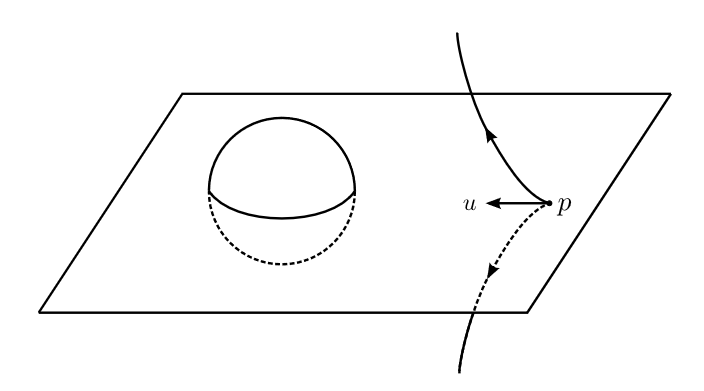
\includegraphics[scale=0.5]{immagini/perassurdo.png}
    \caption{La geodetica deve giacere nello stesso piano altrimenti per simmetria dovrebbe essercene una speculare, generando un assurdo con l'unicità della soluzione noti i dati iniziali.}
    \label{fig.perassurdo}
\end{figure}

Poiché ogni geodetica può essere riportata tramite rotazioni ad una inizialmente equatoriale, possiamo assumere senza perdita di generalità che $\theta = \frac{\pi}{2}$, e ottenere:
\begin{equation*}
    - \varkappa = - \left( 1- \frac{2M}{r}\right) \Dot{t}^2 + \left( 1- \frac{2M}{r}\right)^{-1}\Dot{r}^2 + r^2\Dot{\phi}^2
\end{equation*}

Riscriviamo utilizzando le grandezze conservate dai vettori di Killing, $\Dot{t} = E(1-\frac{2M}{r})^{-1}$ e $\Dot{\phi} = L (r\sin\theta)^{-2}= Lr^{-2}$:
\begin{equation*}
    - \varkappa = -\frac{E^2}{1-\frac{2M}{r}} + \frac{\Dot{r}^2}{1-\frac{2M}{r}} + \frac{L^2}{r^2}
\end{equation*}
cioè riarrangiando:
\begin{equation}
    \frac{E^2}{2} = \frac{\Dot{r}^2}{2} + \frac{1}{2}\left(1-\frac{2M}{r}\right) \left(\frac{L^2}{r^2} + \varkappa \right)
    \label{eq.motoradialegeodschwarz}
\end{equation}

Da un punto di vista classico corrisponde al moto radiale di una particella di massa unitaria non relativistica la quale è sottoposta ad un potenziale efficace:
\begin{align}
    V &= \frac{1}{2}\left(1-\frac{2M}{r}\right) \left(\frac{L^2}{r^2} + \varkappa \right)\nonumber \\
    &=\frac{\varkappa}{2} - \frac{M\varkappa}{r} + \frac{L^2}{2r^2} - \frac{ML^2}{r^3} 
    \label{eq.potenziale_efficace_geodetiche_schwarz}
\end{align}
Osserviamo che tale potenziale è composto da un termine che riconduce al potenziale newtoniano $\frac{M}{r}$, il potenziale centrifugo $\frac{L^2}{2r^2}$ e un ultimo termine di correzione relativistica. Analizziamo quindi il moto al variare di $\varkappa$:
\begin{description}
    \item[Geodetiche tipo tempo]
    Il potenziale assume la forma:
    \begin{equation*}
        V= \frac{1}{2} - \frac{M}{r} + \frac{L^2}{2r^2} - \frac{ML^2}{r^3} 
    \end{equation*}
Ha estremanti per i valori:
    \begin{equation*}
        r_{\pm} = \frac{L^2\pm \sqrt{L^4-12 L^2 M^2}}{2M}
    \end{equation*}
Pertanto se $L^2 < 12M^2$, non ci sono estremi, mentre per $L^2 >12M^2$, $r_+$ è un minimo e $r_-$ è massimo. Questo massimo comporta un'orbita circolare metastabile che non esiste nella teoria newtoniana.
    \item[Geodetiche tipo luce]
    Il potenziale assume la forma:
    \begin{equation*}
        V = \frac{L^2}{2r^2} - \frac{ML^2}{r^3} = \frac{L^2}{r^3}(r-2M)
    \end{equation*}
Si ha un massimo per $r=3M$ a cui corrisponde un'energia pari a $\frac{L^2}{54M^2}$.
\end{description}
I grafici sono mostrati in fig. \ref{fig.geodetiche_schwarz}
\begin{figure}
    \centering
    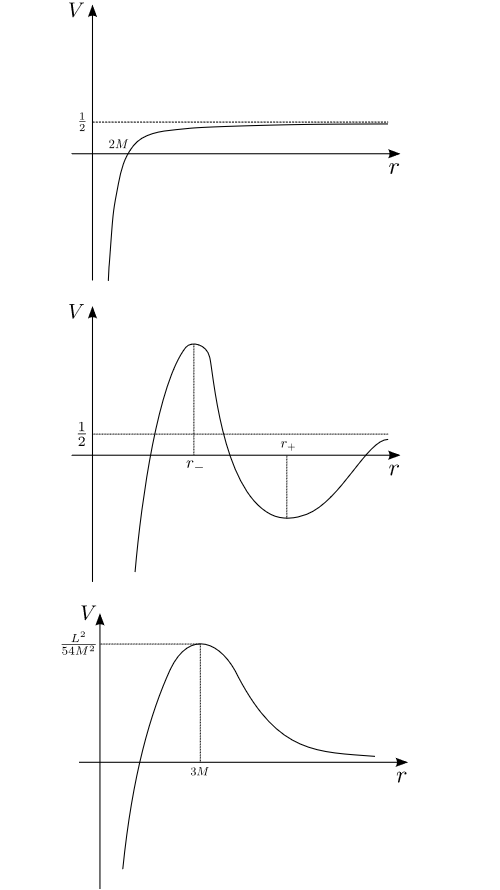
\includegraphics[scale=0.8]{immagini/geodetiche.png}
    \caption{Geodetiche della soluzione di Schwarzschild. Le prime due corrispondo a geodetiche di tipo tempo per $L^2 <12M^2$ e $L^2>12M^2$. L'ultima è la geodetica di tipo luce.}
    \label{fig.geodetiche_schwarz}
\end{figure}
\section{Test classici della relatività generale}
\subsection{Deviazione della luce}
Riprendendo la geodetica di tipo luce prima determinata, si ha per valori di energia
\begin{equation*}
    \frac{E^2}{2} < \frac{L^2}{54M^2}
\end{equation*}
che il moto di un fotone proveniente da infinito, raggiunge un minimo in $r_0$ per poi invertire il suo moto e tornare infinitamente distante, fig. \ref{fig.deflessione}. Questo è il caso di interesse per studiare la deviazione della luce.
\begin{figure}
    \centering
    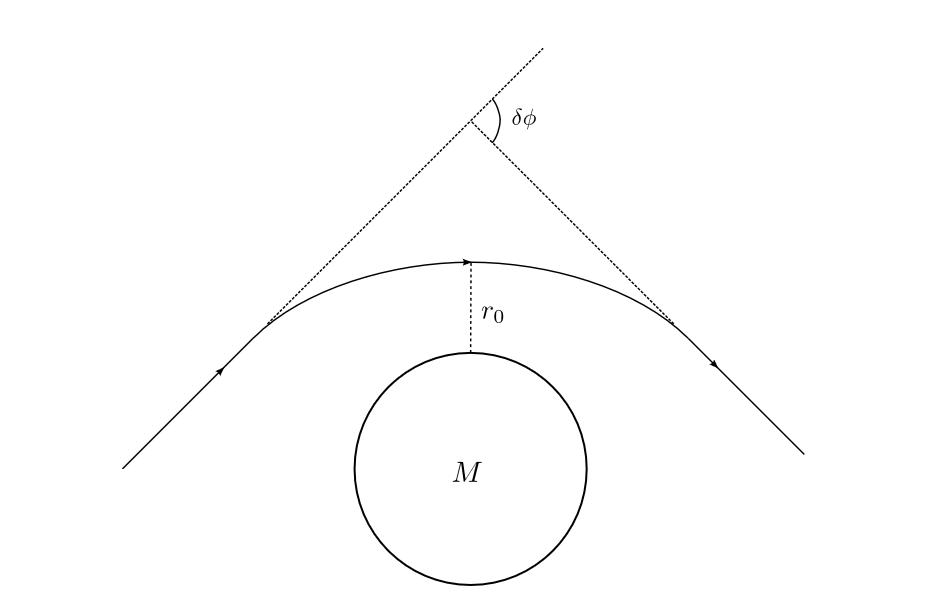
\includegraphics[scale=0.5]{immagini/deflessione.png}
    \caption{Rappresentazione schematica della deflessione della luce.}
    \label{fig.deflessione}
\end{figure}
Definiamo:
\begin{equation*}
    b = \frac{L}{E}
\end{equation*}
detto parametro di impatto apparente. Tale valore in uno spaziotempo piatto corrisponderebbe al parametro di impatto noto nello studio della diffusione, ovvero la distanza minima dall'origine $r=0$; in uno spaziotempo curvo perde questo significato e per tale motivo lo definiamo apparente, sebbene la sua definizione possa rimandare al caso piatto. Questa distanza $r_0$ soddisfa:
\begin{equation*}
    \frac{E^2}{2} = V(r_0) = \frac{L^2}{r_0^3}(r_0 -2M) \iff r_0^3 - b^2(r_0-2M) = 0
\end{equation*}

Consideriamo l'energia del moto radiale eq. \ref{eq.motoradialegeodschwarz}, nel caso della luce cioè con $\varkappa=0$:
\begin{equation*}
    \frac{E^2}{2}= \frac{\Dot{r}^2}{2} + \frac{L^2}{2r^2}-\frac{ML^2}{r^3} \implies \Dot{r}^2 = E^2 - \frac{L^2}{r^2} + \frac{2ML^2}{r^3}
\end{equation*}
Dunque vogliamo esprimere l'angolo al variare del raggio, come in un classico caso di scattering:
\begin{equation*}
    \frac{d\phi}{dr}= \frac{d\phi}{dt}\frac{dt}{dr} = \frac{\Dot{\phi}}{\Dot{r}} = \frac{L}{r^2\sqrt{ E^2 - \frac{L^2}{r^2} + \frac{2ML^2}{r^3} }}
\end{equation*}
Definendo $u=\frac{1}{r}$, si ha $\frac{d\phi}{dr}= \frac{d\phi}{du}\frac{du}{dr} = -\frac{1}{r^2}\frac{d\phi}{du}$ allora:
\begin{equation*}
    \frac{du}{d\phi} = - \frac{1}{L}\sqrt{  E^2 - L^2u^2 +2ML^2u^3    } =- \sqrt{ \frac{1}{b^2} - u^2 +2Mu^3}
\end{equation*}
cioé otteniamo l'equazione differenziale:
\begin{equation}
    u'(\phi)^2 = b^{-2} -u^2 +2Mu^3
    \label{eq.ellitticadeviazioneluce}
\end{equation}
detta \textbf{equazione differenziale ellittica  di Weierstrass}. Come tutte le equazioni differenziali ellittiche, la risoluzione è avanzata e pertanto la risolveremo tramite un metodo perturbativo. Segue:
\begin{equation}
    2u'u" = -2u u' +6Mu^2 u' \implies u" +u = 3Mu^2
    \label{eq.deviazioneluce_perturb}
\end{equation}
Risolviamo il caso imperturbato, cioè in uno spaziotempo piatto con $M=0$; in questo caso i raggi sono delle rette e l'equazione da risolvere è ben nota:
\begin{equation*}
    u" + u = 0 \implies u_0 = C\sin(\phi - \phi_0)
\end{equation*}
Chiamando $u_0$ tale soluzione, si devono imporre le condizioni al contorno che comportano $C=\frac{1}{b}$.

Per risolvere perturbativamente avremo $u= u_0 +\delta u$ che sostituita in eq. \ref{eq.deviazioneluce_perturb} e sfruttando l'identità dell'impertubata:
\begin{equation*}
    u_0"+ \delta u" + u_0 + \delta u = 3M(u_0^2 +(\delta u)^2 +2u_0\delta u)
\end{equation*}
Trascurando inoltre il termine al secondo ordine:
\begin{equation*}
    \delta u" +\delta u =3Mu_0^2 = \frac{3M}{b^2}\sin^2(\phi - \phi_0)
\end{equation*}

Dunque ponendo $\phi_0 = 0$, tale equazione ha soluzione
\begin{equation}
    \delta u = \frac{M}{b^2}(1+ \cos\phi)^2
    \label{eq.deviazione_perturbazione_soluzione}
\end{equation}
così che otteniamo la soluzione totale al primo ordine:
\begin{equation}
    u=\frac{1}{b}\left(  \sin\phi+ \frac{M}{b}(1+\cos\phi)^2 + o(\frac{M}{b})   \right)
    \label{eq.deviazione_totale_soluzione}
\end{equation}

Nel caso del nostro sistema solare $\frac{M}{b} \ll 1$, ed è valido adottare tale soluzione. Il raggio di luce pertanto proviene da infinito e viene deviato dal Sole di un angolo $\delta \phi$ rispetto la direzione incidente e prosegue in traiettoria retta all'infinito; il primo punto (banale) di infinito si ottiene per un angolo $\phi = \pi$ che giustamente comporta $u= 0 \implies r= \infty$. Il secondo punto ad infinito si ottiene sempre annullando $u$, supponendo $\phi_0 = 0$ dell'imperturbata (cioé $\phi = \delta \phi)$:
\begin{equation*}
     \sin\delta\phi+ \frac{M}{b}(1+\cos\delta\phi)^2 = 0
\end{equation*}
ovvero
\begin{equation}
    \delta \phi = - \frac{4M}{b} + o(\frac{M^2}{b^2})
    \label{eq.angolo_deviazione_luce}
\end{equation}
questo corrisponde all'effettivo angolo di deviazione della luce.

\subsection{Redshift gravitazionale}
Consideriamo due osservatori $\mathcal{O}_1$ e $\mathcal{O}_2$, statici, ovvero con quadrivelocità $u_1$, $u_2$ parallele a $\partial_t$: le loro linee di mondo saranno pertanto orbite di $\partial_t$ con posizione $r, \theta, \phi$ fissati, fig. \ref{fig.redshiftgravit}.
Ipotizziamo che $\mathcal{O}_1$ invii dal suo punto $P_1$ un segnale luminoso e che venga ricevuto da $\mathcal{O}_2$ nel punto $P_2$. Il segnale luminoso percorrerà una geodetica di tipo luce per la quale chiamiamo $k^\mu$ il vettore tangente.

\begin{figure}
    \centering
    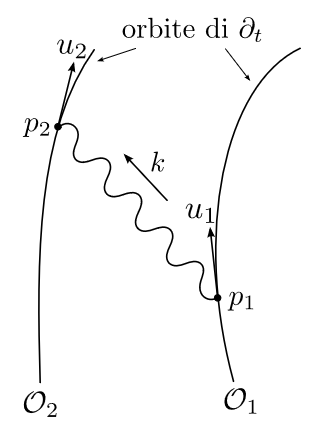
\includegraphics[scale=0.5]{immagini/redshiftgravi.png}
    \caption{Rappresentazione del redshift gravitazionale.}
    \label{fig.redshiftgravit}
\end{figure}
La frequenza di emissione:
\begin{equation*}
    \omega_1 = -k_\mu u^\mu_1 |_{P_1}
\end{equation*}
mentre la frequenza misurata nella ricezione:
\begin{equation*}
    \omega_2 = -k_\mu u^\mu_2 |_{P_2}
\end{equation*}
Poiché le quadrivelocità sono normalizzate, $u_1 ^2 = u_2 ^2 = -1$, e parallele al vettore di Killing $\xi =\partial_t$, potremo scrivere:
\begin{align*}
    u_1^\mu = \frac{\xi^\mu}{(-\xi^2)^{1/2}}\big|_{P_1} &&  u_2^\mu = \frac{\xi^\mu}{(-\xi^2)^{1/2}}\big|_{P_2}
\end{align*}
Si avrà inoltre che
\begin{equation*}
    k \cdot \xi |_{P_1} = k \cdot \xi |_{P_2}
\end{equation*}
poiché lungo la geodetica questa quantità rimane costante. Facendo il rapporto delle frequenze con queste considerazioni si ottiene:
\begin{equation*}
    \frac{\omega_1}{\omega_2} = \frac{ - k_\mu \xi^\mu (-\xi^2)^{-1/2}|_{P_1}}{ - k_\mu \xi^\mu (-\xi^2)^{-1/2}|_{P_2}} = \frac{(-\xi^2)^{-1/2}|_{P_1}}{(-\xi^2)^{-1/2}|_{P_2}}
\end{equation*}
Non resta altro che calcolare il quadrato di $\xi$ nella metrica scelta\footnote{Questa derivazione è valida per un qualsiasi spaziotempo stazionario.}:
\begin{equation*}
    \xi^2 = < \xi, \xi > = < \partial_t, \partial_t > = g_{tt} = - \left( 1-\frac{2M}{r}\right)
\end{equation*}

Otteniamo dunque:
\begin{equation}
    \frac{\omega_1}{\omega_2} = \sqrt{\frac{\left( 1-\frac{2M}{r_2}\right)}{\left( 1-\frac{2M}{r_1}\right)}}
    \label{eq.redshift_frequenze}
\end{equation}

Osserviamo dunque il caso $r_2 > r_1$, cioè l'emettitore più vicino al centro di attrazione gravitazionale, allora si avrà $\omega_2 < \omega_1$ altresì $\lambda_2 > \lambda_1$: la lunghezza d'onda misurata è più lunga rispetto quella emessa, cioè ha subito uno \emph{spostamento verso il rosso} o \emph{redshift}. In altri termini, l'energia del fotone $E=\hbar \omega$ è diminuita poiché è passata in una regione a maggiore potenziale gravitazionale.

Se analizziamo il limite $M \ll r_1, r_2$, eseguendo le opportune approssimazioni con sviluppi di Taylor ed esplicitando le costanti prima mantenute unitarie:
\begin{equation*}
    \frac{\Delta \omega}{\omega} \approx - \frac{GM}{c^2r^1} + - \frac{GM}{c^2r^2} \iff \hbar \Delta \omega \approx \frac{\hbar \omega}{c^2}\left( - \frac{GM}{r^1} + - \frac{GM}{r^2}\right)
\end{equation*}
risulta evidente come la differenza di energia del fotone sia dovuta alla differenza del potenziale gravitazionale newtoniano tra i punti iniziali e finali.

L'effetto fu sperimentalmente verificato nel 1959 da R. Pound e G. Rebka, sfruttando l'effetto Mössbauer nell'emissione di raggi gamma (cioè senza rinculo) da parte di un nucleo di $^{57}$Fe.
Chiariamo infine che questo effetto doppler è ben diverso da quello relativistico, emerso nella relatività ristretta, e trae origine nel principio di equivalenza e nella dilatazione temporale nei pressi del pozzo gravitazionale (la sorgente del campo); è l'effetto doppler che insieme a quello relativistico, vanno tenuti in considerazione nella progettazione dei sistemi di navigazione satellitare. Con osservatore ed emettitore lontani dalle sorgenti di campo, in regime di metrica piatta, il redshift gravitazionale è evidentemente trascurabile.

Esisterà poi un altro tipo di redshift dovuto invece alla struttura dell'universo e alla sua espansione.


\subsection{Precessione del perielio}
Riprendendo i calcoli delle geodetiche di tipo tempo:
\begin{equation*}
    \left(\frac{dr}{d\phi}\right)^2 = \frac{\Dot{r}^2}{\dot{\phi}^2} = \frac{E^2 -1 +\frac{2M}{r} - \frac{L^2}{r^2} + \frac{2ML^2}{r^3}}{\frac{L^2}{r^4}}
\end{equation*}
Introducendo la variabile $u=r^{-1}$ e il parametro d'urto apparente $b = \frac{L}{E}$:
\begin{equation*}
    \left(\frac{du}{d\phi}\right)^2 = b^{-2} - L^{-2} + \frac{2M}{L^2}u - u^2 +2Mu^3 
\end{equation*}
Derivando una volta e semplificando:
\begin{equation*}
    2u'u" = \frac{2M}{L^2} u' - 2u u' +6Mu^2u'
\end{equation*}
otteniamo
\begin{equation}
    u"(\phi) = \frac{M}{L^2} +3Mu^2(\phi) - u(\phi)
    \label{eq.diff_perielio}
\end{equation}
Osserviamo che questa equazione differenziale, rispetto al caso newtoniano, differisce per il termine $3Mu^2$. La sua soluzione esatta è una funzione ellittica, pertanto la risolveremo perturbativamente, così come si è già fatto. I termini di validità dell'approccio perturbativo saranno chiariti in seguito. 

L'equazione imperturbata fornisce la soluzione del problema di Keplero:
\begin{equation}
    u" +u = \frac{M}{L^2} \implies u_0 = \frac{M}{L^2} (1+\epsilon\cos\phi)
    \label{eq.imperturbata_keplero}
\end{equation}
Cercando soluzioni $u= u_0 + \delta u$ in eq. \ref{eq.diff_perielio} e trascurando termini al secondo ordine:
\begin{align}
    u_0" +\delta u" + u_0 + \delta u = \frac{M}{L^2} + 3M(u_0^2+ (\delta u)^2 +2u_0 \delta u) \nonumber \\
    \implies \delta u" + \delta u = 3M u_0^2
    \label{eq.diff_perielio_perturb}
\end{align}
L'approccio perturbativo risulta valido quando $Mu = \frac{M}{r} \ll 1$. Attraverso il metodo della variazione delle costanti si risolve eq. \ref{eq.diff_perielio_perturb} ricavando:
\begin{equation}
    \delta u = \frac{3M^3}{L^4}\left(1 + \epsilon \phi \sin \phi + \epsilon^2(\frac{1}{2} -\frac{1}{6}\cos(2\phi) )\right)
\end{equation}

Il metodo perturbativo ci fornisce dunque:
\begin{equation*}
     u = u_0 + \frac{3M^3}{L^4}\left(1 + \epsilon \phi \sin \phi + \epsilon^2(\frac{1}{2} -\frac{1}{6}\cos(2\phi) )\right)
\end{equation*}
Questa non è più periodica e inoltre possiede un termine dominante illimitato, $\phi\sin\phi$. Trascurando le altre correzioni:
\begin{equation*}
    u = \frac{M}{L^2}\left( 1+\epsilon\cos\phi + \epsilon\frac{3M^2}{L^2}\phi\sin\phi\right)
\end{equation*}
e applicandola al caso $\frac{M}{L} \ll 1$ (questo è ben soddisfatto nel caso solare):
\begin{equation}
    u \approx \frac{M}{L^2}\left( 1+\epsilon\cos((1-3\frac{3M^2}{L^2})\phi)\right)
\end{equation}
In questa approssimazione, la soluzione è nuovamente periodica, ma non più di $2\pi$; non descrive orbite chiuse, ma che precedono al perielio di un angolo $\Delta \phi$ pari a:
\begin{equation}
    \Delta \phi = \frac{2\pi}{1-\frac{3M^2}{L^2}} \approx 2\pi\left(1+\frac{3M^2}{L^2}\right)
    \label{eq.precessione}
\end{equation}
\begin{figure}
    \centering
    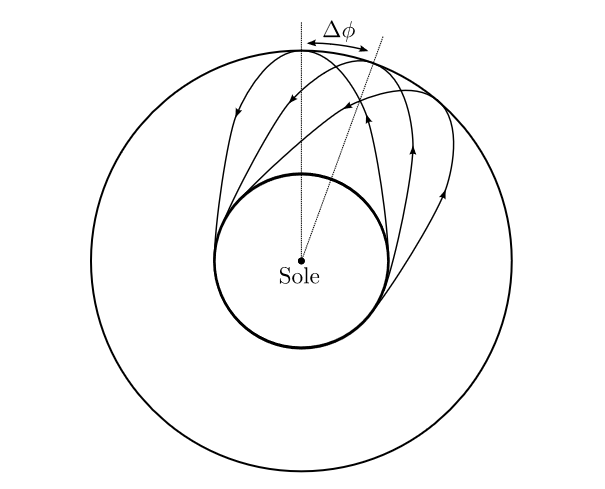
\includegraphics[scale=0.5]{immagini/precessione.png}
    \caption{Rappresentazione schematica della precessione di Mercurio.}
    \label{fig.precessione}
\end{figure}

\section{Estensione di Kruskal}\label{para.kruskal}
Sebbene il concetto di buco nero e orizzonte degli eventi fossero già stati descritti agli albori della relatività generale, dopo che era stata formulata la soluzione di Schwarzschild, si deve a Martin D. Kruskal, in parallelo a George Szekeres, nel 1960, il lavoro che ha permesso di descrivere in maniera completa la singolarità della metrica.
Le prime discussioni di un buco nero in tale metrica erano limitate a descrivere la sola regione al di fuori dell'orizzonte degli eventi (il significato di tale termine sarà poi chiarito); come vedremo quella che prende il nome di \emph{estensione di Kruskal}, fornisce una descrizione più completa e ha permesso l'introduzione di ulteriori concetti quali il \emph{buco bianco} o il \emph{ponte di Einstein-Rosen}.

Riprendendo la soluzione di Schwarzschild, eq. \ref{eq.metricaschwarz}, possiamo vedere come in $r= 2M$, ovvero per il cosiddetto raggio di Schwarzschild, la metrica sia singolare con $g_{tt}\rightarrow 0$ e $g_{rr}\rightarrow+\infty$. Questa non è una \textbf{singolarità di curvatura}, come invece è $r=0$. Ad esempio l'invariante di curvatura:
\begin{equation*}
    R_{\mu\nu\rho\sigma} R^{\mu\nu\rho\sigma} \propto \frac{1}{r^2}
\end{equation*}
detto \emph{scalare di Kretschmann}, è singolare in $r=0$, non in $r=2M$. Il raggio di Schwarzschild è invece una \textbf{singolarità delle coordinate}.

Da un punto di vista fisico, per ogni configurazione statica all'equilibrio, la regione $r\leq 2M$ è interna alla distribuzione di materia e pertanto la sua discussione non è rilevante allo studio del campo gravitazionale di, ad esempio, una stella statica.  Corpi sufficientemente massivi invece, quando esauriscono gli elementi che mantengono attiva la fusione nucleare che avviene in essi e che compensa l'attrazione dovuta all'enorme materia, vanno incontro ad un collasso gravitazionale il quale può portarli ad una supernova, una stella di neutroni o ad un buco nero. In questi casi tale regione diventa rilevante allo studio.

L'idea alla base dell'estensione di Kruskal è che se si considerano le geodetiche, che siano tipo tempo o luce, tendenti alla singolarità $r=2M$, queste vi arrivano con parametro affine finito. Il punto non è all'infinito e ciò suggerisce di assumere tale parametro come nuova coordinata.

Osserviamo che in generale nuove singolarità di coordinate si introducono qualora delle geodetiche si intersechino; tuttavia in due dimensioni, almeno localmente, le geodetiche nulle si dividono in \emph{outgoing} e \emph{ingoing}\footnote{Tali geodetiche sono caratterizzate da $t\pm r = \textrm{cost.}$; col segno $+$ si ha che aumentando $t$, deve diminuire $r$ quindi la geodetica \virgolette{si avvicina} (ingoing). Viceversa con l'altro segno.} e dentro tali classi non sono possibili intersezioni. Le coordinate ricercate saranno costanti lungo queste geodetiche. La corrispondente griglia di coordinate sarà quindi basata sulla geometrica \virgolette{griglia} di geodetiche nulle.

Partiamo studiando la metrica bidimensionale (la parte angolare rimane immutata nella simmetria centrale):
\begin{equation*}
    ds^2 = - \left( 1 - \frac{2M}{r}\right) dt^2 +  \left( 1 - \frac{2M}{r}\right)^{-1} dr^2
\end{equation*}
considerando le geodetiche nulle, $ds^2=0$, ovvero la luce, otteniamo:
\begin{equation*}
    dt =  \pm \left( \frac{r}{r-2M}\right) dr
\end{equation*}
Integrando:
\begin{equation*}
    t = \pm r_* + \textrm{cost.}
\end{equation*}
dove $r_* = r+2M\log(\frac{r}{2M}-1)$; questa è chiamata \textbf{coordinata tartaruga di Regge-Wheeler}\footnote{Il nome si rifà al paradosso di Zeno di Achille e la tartaruga; \virgolette{Sfortunatamente Zeno non sapeva che la serie geometrica fosse convergente}. Infatti $r$ varia lentamente, variando $r_*$ poiché $\frac{dr}{dr_*}\rightarrow 0$ per $r\rightarrow2M$.}. Introducendo le coordinate outgoing e ingoing\footnote{Le coordinate \virgolette{ibride} $(u,r)$ o $(v,r)$ sono dette \emph{coordinate di Eddington-Finkelstein}.}:
\begin{equation*}
    \left\{\begin{array}{c}
         u = t - r_* \\
         v = t + r_*
    \end{array}\right.
\end{equation*}
la metrica diventa:
\begin{equation*}
    ds^2 = -  \left( 1 - \frac{2M}{r}\right)dudv
\end{equation*}
Questa mantiene ancora la singolarità $r=2M$. Qui $r$ è funzione delle $u, v$ implicitamente secondo:
\begin{equation*}
    r_*(r)= \frac{v-u}{2}
\end{equation*}
Rielaboriamo la metrica riscrivendo:
\begin{equation*}
    -\left( 1 - \frac{2M}{r}\right) = - \frac{2M}{r}\left( \frac{r}{2M}-1\right)
\end{equation*}
e inoltre:
\begin{equation*}
    \frac{r_*}{2M} = \frac{r}{2M}+\log(\frac{r}{2M}-1) \implies e^{r_*/2M} = e^{r/2M}\left(\frac{r}{2M}-1\right) \implies \left(\frac{r}{2M}-1\right) =  e^{r_*/2M} e^{-r/2M}
\end{equation*}
Comporta:
\begin{equation*}
    ds^2 = - \frac{2M}{r}\exp({-\frac{r}{2M}}) \exp({\frac{v-u}{4M}})dudv
\end{equation*}
Questa metrica è ancora singolare in $r=2M$ cioè $r_*\rightarrow-\infty$ a cui corrispondono $u\rightarrow -\infty$ e $v \rightarrow +\infty$. Tuttavia ci suggerisce le nuove coordinate:
\begin{align}
    U= - e^{-u/4M} && V= e^{v/4M}
\end{align}
dette \textbf{coordinate di Kruskal-Szekeres}. Queste, come da idea iniziale, sono parametri affini per le geodetiche nulle considerate. Osserviamo inoltre che per loro definizione $U<0$ e $V>0$, mentre la singolarità $r=2M$ corrisponde a $U=V=0$. 
Ricalcolando:
\begin{equation*}
    \left\{\begin{array}{l}
    dU = -\frac{U}{4M}du \\ \\
    dV = \frac{V}{4M}dv
    \end{array}\right.  \implies dudv = - 16M^2 \exp{(-\frac{v-u}{4M})}dUdV
\end{equation*}
e la metrica diventa:
\begin{equation}
    ds^2 = -\frac{32M^3 e^{-r/2M}}{r}dUdV
    \label{eq.metrica_kruskal_UV}
\end{equation}
Questa metrica \textbf{non è più singolare} e ci permette di estendere la soluzione di Schwarzschild a tutti i valori $U<0, V>0$ compatibili con $r>0$. Per quanto detto inizialmente, non si può andare con valori oltre $r=0$ perché questo punto rappresenta una singolarità di curvatura.

Effettuiamo infine la trasformazione:
\begin{align}
    T=\frac{U+V}{2} && X=\frac{V-U}{2}
    \label{eq.coordinateTX_kruskal}
\end{align}
così che $dU=dT+dX$ e $dV=dT-dX$ e si ottiene la metrica finale\footnote{Si può fare un'analoga derivazione, che risulta formalmente identica a questa, a partire dalla metrica di Rindler $ds^2 = -x^2dt^2 + dx^2$ che ci permette di dire che l'estensione dello spaziotempo di Rindler è lo spaziotempo di Minkowski.} (riportando anche la parte angolare):
\begin{equation}
    ds^2 = \frac{32M^3 e^{-r/2M}}{r}( - dT^2 + dX^2) + r^2(d\theta^2 + \sin^2\theta d\phi^2)
    \label{eq.metrica_kruskal}
\end{equation}
a meno di un prefattore (che diventa ininfluente per geodetiche nulle), i primi due termini in $T, X$ non sono altro che la metrica di Minkowski, mentre la parte restante è dovuta alla simmetria centrale. Pertanto in un piano $(X,T)$ ogni punto non è altro che una 2-sfera. Esprimiamo la relazione tra le coordinate iniziali $(t,r)$ e $(T,X)$:
\begin{equation}
    \left\{ \begin{array}{l}
          \left(\frac{r}{2M}-1\right) e^{r/2M} = X^2 - T^2 \\
          \frac{t}{2M}= 2\arctanh (\frac{T}{X})
    \end{array}\right.
\end{equation}
In questo modo possiamo rappresentare:
\begin{itemize}
    \item $r=\textrm{cost.} \implies X^2 - T^2 = \textrm{cost.}$ ovvero  un'iperbole.
    \item $r=2M \implies X^2 = T^2$ ovvero le bisettrici.
    \item $t=\textrm{cost.} \implies \frac{T}{X} = \textrm{cost.}$ ovvero delle rette.
    \item $r>0 \implies X^2-T^2 > -1$ ovvero il range di soluzioni permesse.
\end{itemize}
Con queste possiamo quindi rendere graficamente lo spaziotempo di Schwarzschild esteso in presenza di un buco nero come in fig. \ref{fig.kruskal}.
\begin{figure}
    \centering
    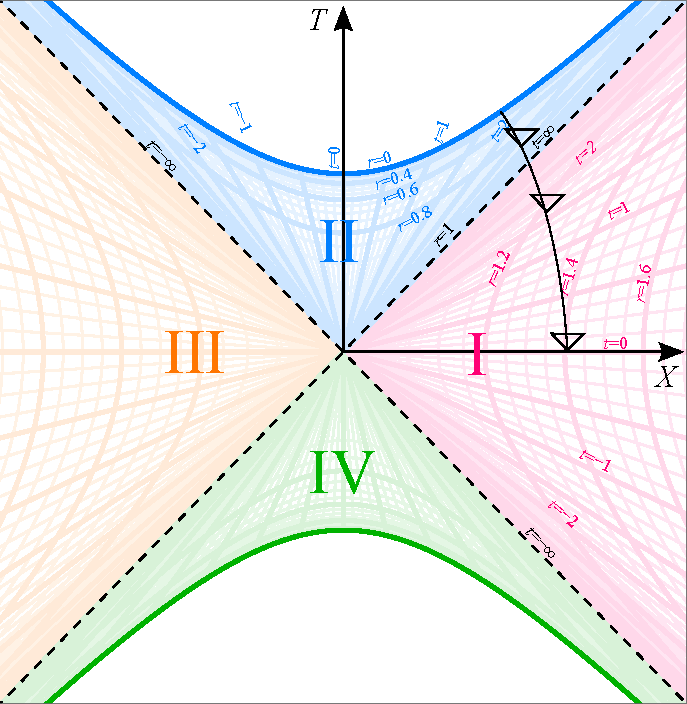
\includegraphics[scale=0.8]{immagini/kruskal.pdf}
    \caption{Spaziotempo di Schwarzschild nell'estensione di Kruskal. Ogni punto del piano rappresenta una 2-sfera. Viene rappresentato un evento che superando l'orizzonte degli eventi, cioè entrando nella regione II, non può più uscirne in quanto la velocità massima che può raggiungere, pari a $c$, non è sufficiente a tagliare la bisettrice (il cono dovrebbe avere un angolo maggiore di 45 gradi).}
    \label{fig.kruskal}
\end{figure}
Per quanto detto sul prefattore della metrica, essendo ininfluente per geodetiche luce, si avrà che i coni di luce saranno comunque a 45 gradi.
Vengono riconosciute 4 regioni; analizziamole:
\begin{description}
    \item[Regione I] corrispondente a $r> 2M$, è la regione asintoticamente piatta che descrive il campo gravitazionale al di fuori della distribuzione di materia sferica.
    \item[Regione II] corrispondente al \textbf{buco nero}, infatti un qualsiasi osservatore che oltrepassi radialmente la bisettrice $X=T$ sarà destinato a cadere nella singolarità rappresentata dalla regione delimitata dall'iperbole superiore. Qualsiasi segnale luminoso inviato dalla regione II sarà destinato a rimanere intrappolato in essa in quanto per intersecare nuovamente la bisettrice, bisognerebbe avere un segnale luminoso con angolo maggiore di 45 gradi, il che non è possibile. La caduta nella singolarità avviene in un intervallo di tempo proprio finito. La bisettrice $X=T$ è chiamata $H^+$ oppure \textbf{orizzonte degli eventi}.
    \item[Regione III] corrispondente ad un altro universo asintoticamente piatto che giace \virgolette{all'interno} del \virgolette{raggio} $r=2M$.
    \item[Regione IV] corrispondente al \textbf{buco bianco}. \'E una regione con il \virgolette{tempo rovesciato} rispetto la regione II. Qualsiasi osservatore all'interno di essa deve necessariamente provenire dalla singolarità $r=0$ e uscirne, attraversando la bisettrice $X=-T$, in un tempo proprio finito. La bisettrice è detta $H^-$ oppure \textbf{orizzonte del passato}.
\end{description}

Per capire la geometria che collega le due regioni I, III si considera la superficie di tipo spazio $T=0$.
La metrica indotta su questa superficie è:
\begin{equation*}
    ds^2 = \left( 1- \frac{2M}{r}\right)^{-1} dr^2 + r^2(d\theta^2 + \sin^2\theta d\phi^2)
\end{equation*}
Grazie alla simmetria sferica possiamo limitarci a discutere il piano equatoriale $\theta= \frac{\pi}{2}$:
\begin{equation}
    ds^2 = \left( 1- \frac{2M}{r}\right)^{-1} dr^2 +r^2 d\phi^2
    \label{eq.metrica_ponte}
\end{equation}
Per visualizzare questa superficie 2-dim., la immergiamo nello spazio euclideo $\mathbb{E}^3$. La metrica standard di $\mathbb{E}^3$ in coordinate cilindriche è:
\begin{equation*}
    ds^2 = dz^2 +dr^2 +r^2d\phi^2
\end{equation*}
Se si considera $z=z(r)$, quindi una superficie di rotazione di $\mathbb{E}^3$, tale metrica indotta su questa superficie è:
\begin{equation*}
    ds^2 = \left[ 1+ \left( \frac{dz}{dr}\right)^2 \right]dr^2 +r^2d\phi^2
\end{equation*}
Abbiamo quindi tutti gli elementi per confrontarla con eq. \ref{eq.metrica_ponte} e visualizzare l'embedding reso possibile da:
\begin{equation*}
    r= 2M + \frac{z^2}{8M}
\end{equation*}
Questo viene chiamato \textbf{ponte di Einstein-Rosen}.
La topologia di tale superficie è $\mathbb{R}\times S^2$; nel grafico una dimensione è necessariamente soppressa, pertanto ogni cerchio rappresenta in realtà una 2-sfera.
Osserviamo inoltre che non è possibile comunicare tra queste due regioni proprio perché qualsiasi segnale luminoso inviato, cadrebbe nel buco nero.

L'estensione di Kruskal descrive uno spaziotempo con buco nero eterno e nel quale compaiono due universi tra loro legati dalla singolarità. In generale non c'è ragione per credere che tale configurazione iniziale sia quella di ogni parte nel nostro universo e pertanto non c'è motivo per pensare che ogni regione dell'universo corrisponda alla completa estensione della soluzione di Schwarzschild. Inoltre se si considera il meccanismo che può portare alla formazione di un buco nero -- collasso gravitazionale --, le regioni III, IV, non si formano nemmeno.

Un corpo sufficientemente massivo che va incontro ad un collasso gravitazionale completo avrà una metrica interna ad esso che non potrà essere quella di Schwarzschild, in quanto $T_{\mu\nu}\neq 0$; tuttavia se consideriamo la regione esterna ad esso, vale Schwarzschild poiché, come visto dal teorema di Birkhoff, è l'unica soluzione a simmetria sferica nel vuoto. Le regioni III, IV sarebbero \virgolette{coperte} dalla materia dell'oggetto in collasso, mentre la regione II verrebbe a crearsi qualora la coordinata radiale diventasse minore di $2M$.

\section{Coordinate di Painlevè-Gullstrand per moto di caduta libera}
Consideriamo un osservatore di tipo tempo in caduta libera nella geometria di Schwarzschild, eq. \ref{eq.metricaschwarz}. Il moto avviene con $\theta, \phi$ costanti e considerando come condizione iniziale $\dot{r}= 0$ per $r\rightarrow + \infty$, ovvero che il moto parta con velocità nulla.

Riprendendo i calcoli effettuati in \S\ref{para.geodschwarz}, il vettore tangente alla geodetica $u^\mu = \frac{d x^\mu}{d\tau} =: x^\mu$ (parametrizzata con tempo proprio) si conserva lungo la stessa e ci ha permesso di scrivere:
\begin{equation*}
    u_\mu(\partial_t)^\mu = - E \implies \dot{t} = E\left( 1 - \frac{2M}{r}\right)^{-1}
\end{equation*}
La condizione di normalità della quadrivelocità ha comportato (considerando $\theta,\phi$ costanti):
\begin{equation}
    -\left( 1 - \frac{2M}{r}\right)\dot{t}^2 + \left( 1 - \frac{2M}{r}\right)^{-1}\dot{r^2} = -1
    \label{eq.normalizza_gullstrand}
\end{equation}
Sostituendo $\dot{t}$ in quest'ultima e riarrangiando otteniamo:
\begin{equation*}
    \dot{r}^2 = E^2 -1 +\frac{2M}{r}
\end{equation*}

Poiché $E$ è costante lungo la geodetica, il suo valore viene determinato dalle condizioni iniziali a $r\rightarrow +\infty$ per le quali si ha $\dot{r}= 0 \implies p = 0$. In questo modo:
\begin{equation*}
    E = \sqrt{p^2 + m^2} \implies E = 1
\end{equation*}
considerando $m = 1$ la massa dell'osservatore test. Pertanto:
\begin{align}
    \dot{t} = \left( 1 - \frac{2M}{r}\right)^{-1} && \dot{r}^2 = \frac{2M}{r}
    \label{eq.dot_gull}
\end{align}

Nell'ipotesi $\dot{r}< 0$ i.e. $\dot{r} = - \sqrt{\frac{2M}{r}}$, se sostituiamo una volta eq. \ref{eq.dot_gull} in eq. \ref{eq.normalizza_gullstrand}, otteniamo:
\begin{equation*}
    \dot{t} + \sqrt{\frac{2M}{r}}\left( 1 - \frac{2M}{r}\right)^{-1}\dot{r} = 1
\end{equation*}
Richiamando $\frac{d x^\mu}{d\tau}$:
\begin{equation}
    dt + \sqrt{\frac{2M}{r}}\left( 1 - \frac{2M}{r}\right)^{-1} dr = d\tau
    \label{eq.dtau_gull}
\end{equation}
ovvero
\begin{equation*}
    \tau = t  + \int_{+\infty}^{r} \sqrt{\frac{2M}{r'}}\left( 1 - \frac{2M}{r'}\right)^{-1} dr'
\end{equation*}

Se usassimo $\tau$ come nuova variabile temporale e sostituissimo $dt$ da eq. \ref{eq.dtau_gull} in eq. \ref{eq.metricaschwarz}, svolgendo il quadrato e semplificando, otterremmo:
\begin{equation}
    ds^2 = - \left( 1 - \frac{2M}{r}\right) d\tau^2 + 2\sqrt{\frac{2M}{r}}d\tau dr + dr^2 + r^2(\sin^2\theta d\phi^2 + d\theta^2)
    \label{eq.metrica_paingull}
\end{equation}
Questa è detta \textbf{metrica di Painlevé-Gullstrand}; si può notare che è stazionaria, ma non statica. Notiamo inoltre che le ipersuperfici $\tau = \textrm{cost.}$ riducono la metrica a quella di $\mathbb{E}^3$, cioè sono ipersuperfici piatte.